% UViT-branch DeepONet (model/uvit_don.py) with the default preset
% configs/beltrami_don_config.py:beltrami_don_sfcqr.
% Compile: pdflatex uvit_don_architecture.tex
\documentclass[tikz,border=6pt]{standalone}
\usepackage{amsmath,amssymb}
\usetikzlibrary{positioning,arrows.meta,calc,fit,backgrounds}

\definecolor{cIn}{HTML}{E8E8E8}
\definecolor{cConv}{HTML}{CFE2F3}
\definecolor{cAttn}{HTML}{F9CB9C}
\definecolor{cEmb}{HTML}{D9EAD3}
\definecolor{cTrunk}{HTML}{EAD1DC}
\definecolor{cHead}{HTML}{FFF2CC}

\tikzset{
  >={Stealth[length=2.2mm]},
  every node/.style={font=\small},
  blk/.style={draw, rounded corners=2pt, align=center, inner sep=3pt},
  % feature map: height ~ spatial resolution
  fmap/.style={blk, minimum width=1.5cm},
  arr/.style={->, thick},
  film/.style={->, densely dashed, thick, green!45!black},
  lbl/.style={font=\scriptsize, inner sep=1pt},
  op/.style={draw, circle, inner sep=1pt, minimum size=6mm, thick},
  sblk/.style={blk, font=\scriptsize, minimum height=6mm},
}

\begin{document}
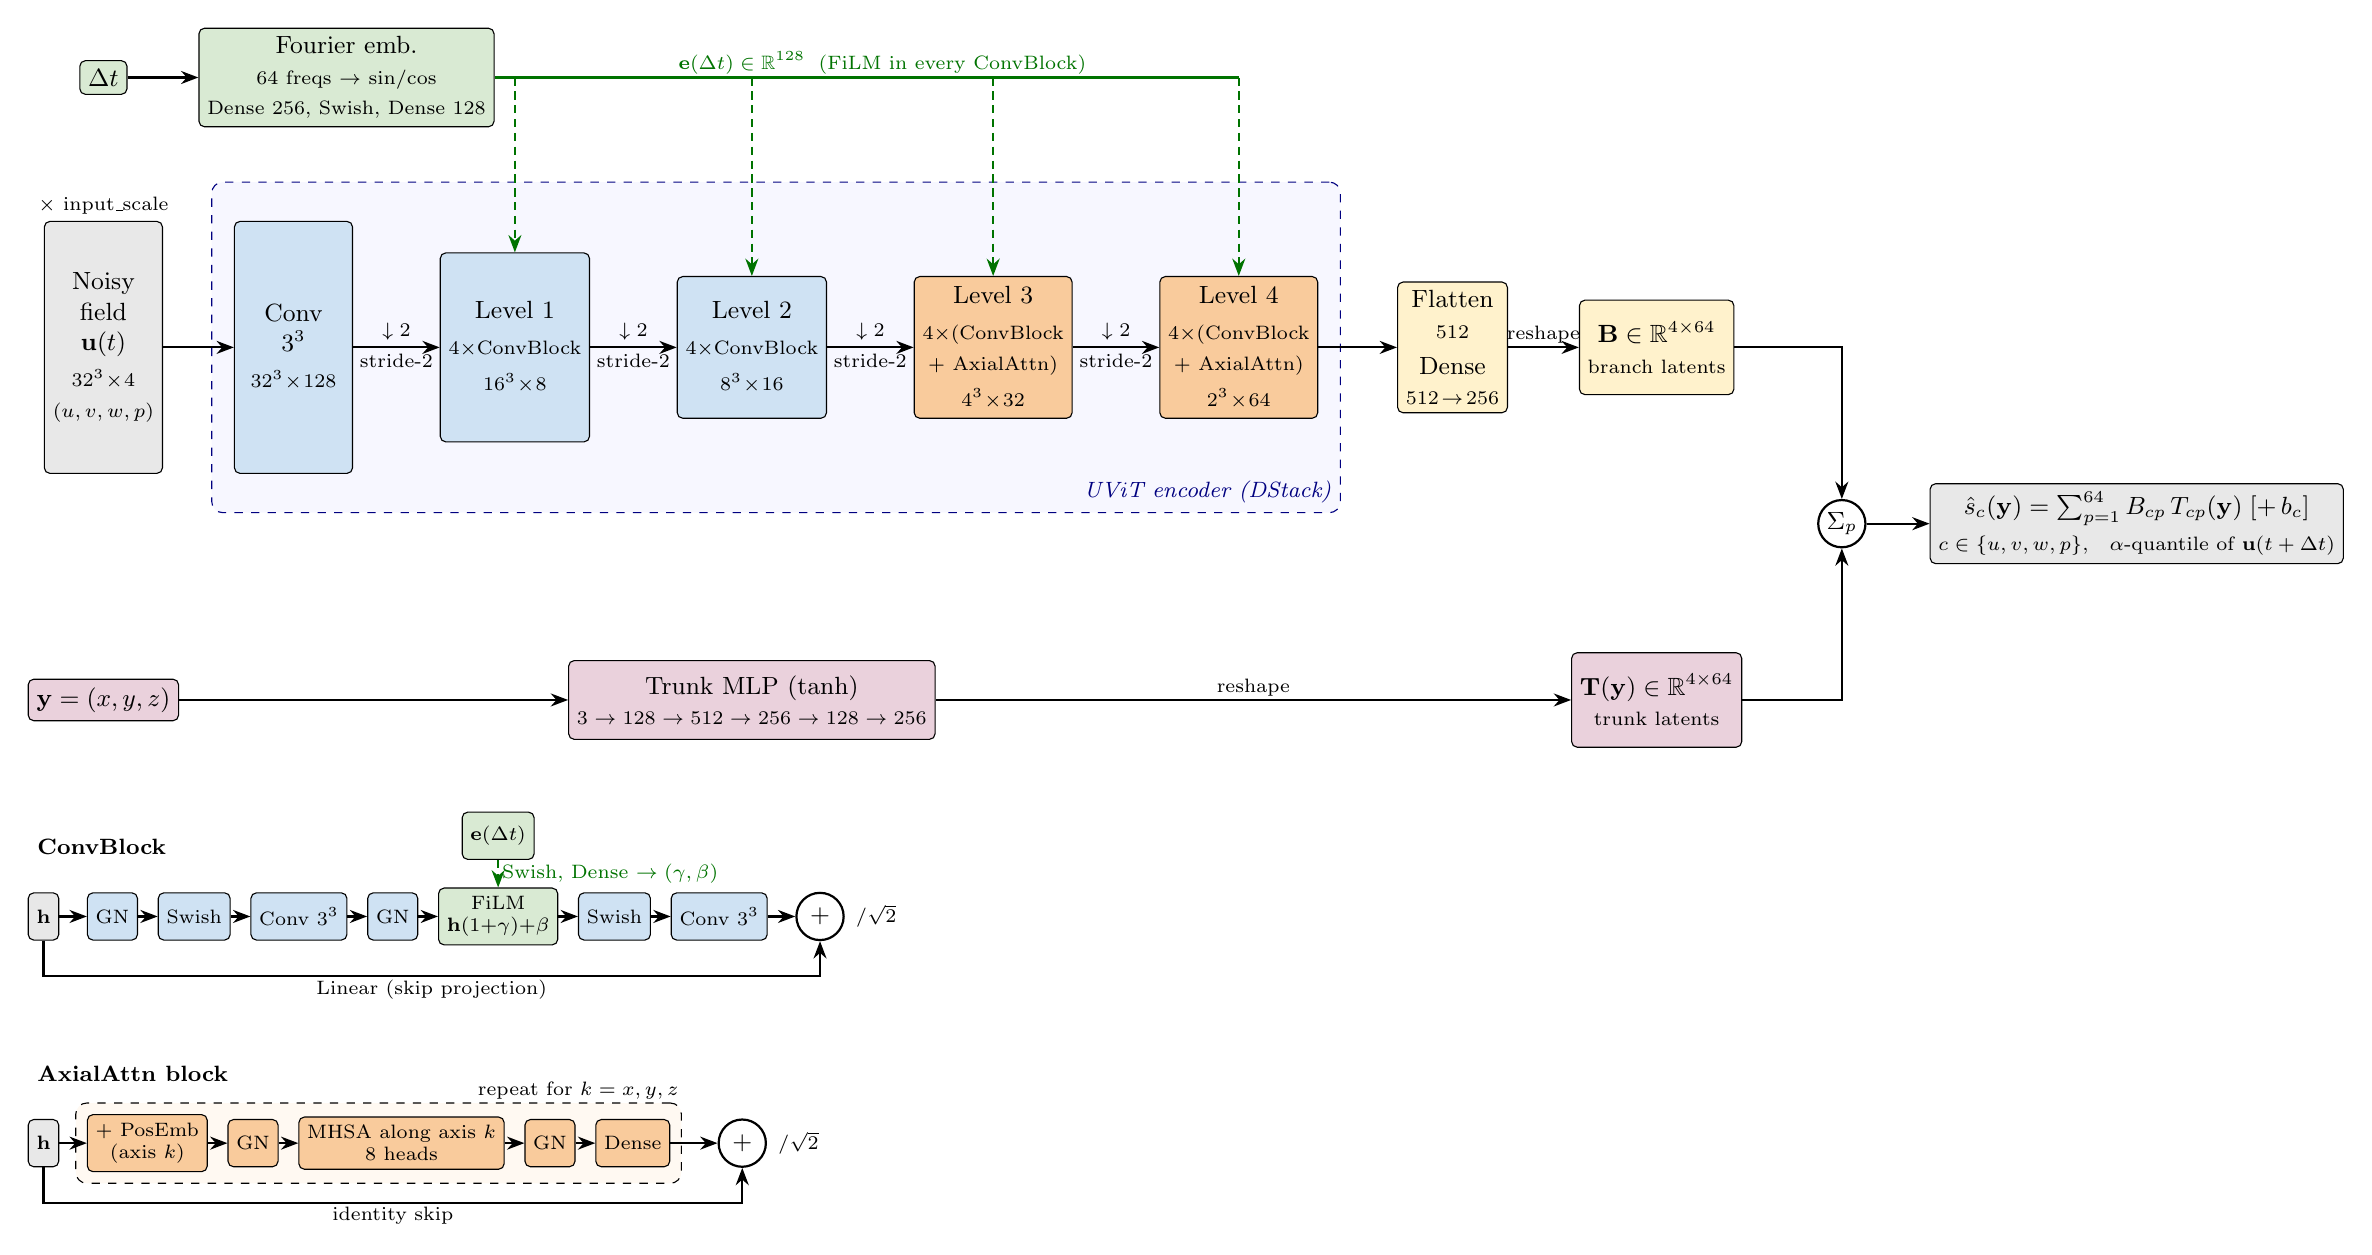
\begin{tikzpicture}

%% ---------------- Branch: UViT encoder ----------------
\node[fmap, fill=cIn, minimum height=3.2cm] (in)
  {Noisy\\field\\$\mathbf{u}(t)$\\[2pt]\scriptsize$32^3\!\times\!4$\\\scriptsize$(u,v,w,p)$};

\node[fmap, fill=cConv, minimum height=3.2cm, right=0.9cm of in] (cin)
  {Conv\\$3^3$\\[2pt]\scriptsize$32^3\!\times\!128$};

\node[fmap, fill=cConv, minimum height=2.4cm, right=1.1cm of cin] (l1)
  {Level 1\\[2pt]\scriptsize$4\times$ConvBlock\\[2pt]\scriptsize$16^3\!\times\!8$};

\node[fmap, fill=cConv, minimum height=1.8cm, right=1.1cm of l1] (l2)
  {Level 2\\[2pt]\scriptsize$4\times$ConvBlock\\[2pt]\scriptsize$8^3\!\times\!16$};

\node[fmap, fill=cAttn, minimum height=1.8cm, right=1.1cm of l2] (l3)
  {Level 3\\[2pt]\scriptsize$4\times$(ConvBlock\\\scriptsize+ AxialAttn)\\[2pt]\scriptsize$4^3\!\times\!32$};

\node[fmap, fill=cAttn, minimum height=1.8cm, right=1.1cm of l3] (l4)
  {Level 4\\[2pt]\scriptsize$4\times$(ConvBlock\\\scriptsize+ AxialAttn)\\[2pt]\scriptsize$2^3\!\times\!64$};

\node[blk, fill=cHead, right=1.0cm of l4, minimum height=1.4cm] (head)
  {Flatten\\\scriptsize$512$\\[2pt]Dense\\\scriptsize$512\!\to\!256$};

\node[blk, fill=cHead, right=0.9cm of head, minimum height=1.2cm] (B)
  {$\mathbf{B}\in\mathbb{R}^{4\times 64}$\\\scriptsize branch latents};

\draw[arr] (in) -- (cin);
\foreach \a/\b in {cin/l1, l1/l2, l2/l3, l3/l4}
  \draw[arr] (\a) -- node[lbl, above=1pt] {$\downarrow 2$} node[lbl, below=1pt] {stride-2} (\b);
\draw[arr] (l4) -- (head);
\draw[arr] (head) -- node[lbl, above] {reshape} (B);

\node[lbl, above=1pt of in] {$\times$ input\_scale};

% Branch frame
\begin{scope}[on background layer]
  \node[draw=blue!50!black, dashed, rounded corners, fill=blue!3,
        inner xsep=8pt, inner ysep=14pt, fit=(cin)(l1)(l2)(l3)(l4)] (dstack) {};
\end{scope}
\node[anchor=south east, font=\footnotesize\itshape, text=blue!50!black]
  at (dstack.south east) {UViT encoder (DStack)};

%% ---------------- Time embedding (FiLM) ----------------
\node[blk, fill=cEmb, above=1.6cm of in] (dt) {$\Delta t$};
\node[blk, fill=cEmb, right=0.9cm of dt] (four)
  {Fourier emb.\\\scriptsize $64$ freqs $\to$ sin/cos\\\scriptsize Dense 256, Swish, Dense 128};
\draw[arr] (dt) -- (four);
\coordinate (bus) at ($(four.east)+(0.4,0)$);
\draw[thick, green!45!black] (four.east) -- (bus) -- (bus -| l4.center);
\node[lbl, text=green!45!black, above] at ($(bus)!0.5!(bus -| l4.center)$)
  {$\mathbf{e}(\Delta t)\in\mathbb{R}^{128}$ \;(FiLM in every ConvBlock)};
\foreach \l in {l1,l2,l3,l4}
  \draw[film] (bus -| \l.center) -- (\l.north);

%% ---------------- Trunk ----------------
\node[blk, fill=cTrunk, below=2.6cm of in] (y) {$\mathbf{y}=(x,y,z)$};
\node[blk, fill=cTrunk, minimum height=1.0cm] (mlp) at (y -| l2.center)
  {Trunk MLP (tanh)\\\scriptsize $3\to128\to512\to256\to128\to256$};
\node[blk, fill=cTrunk, minimum height=1.2cm] (T) at (y -| B.center)
  {$\mathbf{T}(\mathbf{y})\in\mathbb{R}^{4\times 64}$\\\scriptsize trunk latents};
\draw[arr] (y) -- (mlp);
\draw[arr] (mlp) -- node[lbl, above] {reshape} (T);

%% ---------------- Combination ----------------
\coordinate (mid) at ($(B.east)!0.5!(T.east)$);
\node[op, right=1.0cm of mid] (dot) {$\Sigma_p$};
\draw[arr] (B.east) -| (dot.north);
\draw[arr] (T.east) -| (dot.south);
\node[blk, fill=cIn, right=0.8cm of dot] (out)
  {$\hat s_c(\mathbf{y}) = \sum_{p=1}^{64} B_{cp}\,T_{cp}(\mathbf{y}) \;[+\,b_c]$\\[2pt]
   \scriptsize $c\in\{u,v,w,p\}$, \; $\alpha$-quantile of $\mathbf{u}(t+\Delta t)$};
\draw[arr] (dot) -- (out);

%% ---------------- Detail: ConvBlock ----------------
\coordinate (dA) at ($(y.south west)+(0,-1.6)$);
\node[anchor=west, font=\footnotesize\bfseries] (cbt) at (dA) {ConvBlock};
\node[sblk, fill=cIn, below=0.35cm of cbt.south west, anchor=north west] (c0) {$\mathbf{h}$};
\node[sblk, fill=cConv, right=0.35cm of c0] (c1) {GN};
\node[sblk, fill=cConv, right=0.25cm of c1] (c2) {Swish};
\node[sblk, fill=cConv, right=0.25cm of c2] (c3) {Conv $3^3$};
\node[sblk, fill=cConv, right=0.25cm of c3] (c4) {GN};
\node[sblk, fill=cEmb,  right=0.25cm of c4] (c5) {FiLM\\$\mathbf{h}(1{+}\gamma){+}\beta$};
\node[sblk, fill=cConv, right=0.25cm of c5] (c6) {Swish};
\node[sblk, fill=cConv, right=0.25cm of c6] (c7) {Conv $3^3$};
\node[op, right=0.35cm of c7] (c8) {$+$};
\node[lbl, right=0.1cm of c8] {$/\sqrt2$};
\foreach \a/\b in {c0/c1,c1/c2,c2/c3,c3/c4,c4/c5,c5/c6,c6/c7,c7/c8}
  \draw[arr] (\a) -- (\b);
\draw[arr] (c0.south) -- ++(0,-0.45) -| node[lbl, pos=0.25, below] {Linear (skip projection)} (c8.south);
\node[sblk, fill=cEmb, above=0.35cm of c5] (embin) {$\mathbf{e}(\Delta t)$};
\draw[film] (embin) -- node[lbl, right] {Swish, Dense $\to(\gamma,\beta)$} (c5);

%% ---------------- Detail: Axial attention block ----------------
\node[anchor=west, font=\footnotesize\bfseries] (abt)
  at ($(c0.west)+(0,-2.0)$) {AxialAttn block};
\node[sblk, fill=cIn, below=0.35cm of abt.south west, anchor=north west] (a0) {$\mathbf{h}$};
\node[sblk, fill=cAttn, right=0.35cm of a0] (a1) {+ PosEmb\\(axis $k$)};
\node[sblk, fill=cAttn, right=0.25cm of a1] (a2) {GN};
\node[sblk, fill=cAttn, right=0.25cm of a2] (a3) {MHSA along axis $k$\\8 heads};
\node[sblk, fill=cAttn, right=0.25cm of a3] (a4) {GN};
\node[sblk, fill=cAttn, right=0.25cm of a4] (a5) {Dense};
\node[op, right=0.6cm of a5] (a6) {$+$};
\node[lbl, right=0.1cm of a6] {$/\sqrt2$};
\foreach \a/\b in {a0/a1,a1/a2,a2/a3,a3/a4,a4/a5,a5/a6}
  \draw[arr] (\a) -- (\b);
\begin{scope}[on background layer]
  \node[draw, dashed, rounded corners, fill=orange!5, inner sep=4pt,
        fit=(a1)(a5)] (loop) {};
\end{scope}
\node[lbl, anchor=south east] at (loop.north east) {repeat for $k = x, y, z$};
\draw[arr] (a0.south) -- ++(0,-0.45) -| node[lbl, pos=0.25, below] {identity skip} (a6.south);

\end{tikzpicture}
\end{document}
